\subsection{Założenia teorytyczne}
\subsubsection{Semantyczne a syntaktyczne reprezentacje audio w wektorach cech}
Dla proponowanego przez nas rozwiązanie, potencjalnie najważniejszą charakterystyką, którą wykazują się dostępne modele ASR jest postać ukrytej (latentnej) reperezentacji enkodowanej przez nie na podstawie danych wejściowych. Potencjalnie, większa wierność semantycznemu znaczeniu wypowiedzianego zdania doprowadzi do dokładniejszej translacji wyjścia enkodera na współdzielną przestrzeń embeddingów, czego konsekwencją będą lepsze osiągi systemu wyszukiwania dla użytkownika końcowego.
\subsubsection{Wpływ charakterystyki wektorów cech na jakość embeddingów w modelach wielojęzykowych}
Kolejnym aspektem ewaluowanym przez nas w ramach eksperymentu są podobieństwa wyników modeli dla zdań o tym samym znaczeniu w kilku językach. Dla modeli enkodujących semantykę danych, reprezentacje dla dwóch znaczeniowo identycznych zdań w dwóch różnych językach powinny być do siebie podobne według przyjętej metryki podobieństwa. Przykładowo, miara podobieństwa dla reprezentacji latentnych dla zdań "Kocham zwiedzać włoskie miasta" i "I love sightseeing Italian cities", dla modelu semantycznego, powinna mieć jak największą wartość.

Należy mieć na uwadze, że różnice w historii języka, jego strukturze i alfabecie istotnie wpływają na otrzymane wyniki podobieństwa dla takich zdań. Zróżnicowanie to zostało zbadane przez Aleshinę et. al w ich pracy ewaluującej rozkłady embeddingów zdań dla dziesięciu różnych języków \cite{multilanguageEmbeddingDifferences}. Korzystając z modelu MUSE \cite{museModel} operującego na pojedynczych słowach, wykazali oni znaczące pokrycie klastrów embeddingów dla języków o podobnej historii (arabski i hiszpański) jak i o podobnie prostej morfologii i częściowo współdzielonym słownictwie (angielski, chiński, indonezyjski), i izolację klastrów dla wybranych języków (rosyjski, o innym alfabecie i bardziej skomplikowanej morfologii w świetle inflekcji języka). Najbardziej interesującym dla nas wnioskiem są podobieństwa dla słów zapożyczonych z innych języków -- wiele terminów medycznych wywodzi się z języka łacińskiego, co oznacza potencjalnie wysokie podobieństwo dla takich zwrotów w języku angielskim i polskim, jak i w innych językach \cite{latinMedical}.

Wysoka miara podobieństwa dla modelu ASR ewaluowanego dla danych wielojęzykowych oznaczałaby nie tylko dobre radzenie sobie z samą semantyką wypowiedzianych zdań, lecz także potencjalnie wysoki potencjał do przeprowadzenia treningu modelu na specjalistycznych danych dostępnych w innych językach. Model wykazujący się taką cechą byłby niezwykle cenny dla poprawienia jakości wyszukiwania informacji dla nie tylko polskojęzycznych, ale również innych języków wspieranych przez ten model. Właśnie taki proces destylacji wiedzy zbadali w swojej pracy Piperno et. al \cite{multilingualDomainTranslation}, z powodzeniem korzystając z anglojęzycznych zbiorów słownictwa o tematyce medycznej do poprawienia osiągów modeli dla danych w językach hiszpańskim, niemieckim i francuskim. Przeprowadzony w ten sposób dodatkowy trening pozwoliłaby nam na znaczące polepszenie naszego całościowego rozwiązania, umożliwiając skorzystanie z większej ilości danych dostępnych w języku angielskim i przełożenia zdobytej przez model wiedzy na język polski dla zbioru ADMEDVoice \cite{ADMEDVoice}.


\subsection{Metodologia}
\subsubsection{Ocena jakości embeddingów}
W celu rzetelenej weryfikacji powyższej hipotezy dotyczącej semantyki w reprezentacjach latentnych modeli ASR, sformułowaliśmy eksperyment wykorzystujący istniejące modele embeddingowe dla tekstu wspierające wiele języków. Wykorzystując istniejące zbiory danych zawierające zarówno audio wypowiedzianego zdania, jak i jego transkrypcję, za ich pomocą wygenerowaliśmy przykłady treningowe dla każdego zdania inspirowane metodą \textit{triplet loss} \cite{tripletLoss}.

\begin{equation}
    \mathcal{L}_{\text{triplet}} = \max \Big( 0, \; \| f(x^a) - f(x^p) \|_2^2 - \| f(x^a) - f(x^n) \|_2^2 + \alpha \Big)
    \label{eq:tripletloss}
\end{equation}

Na początku dla transkrypcji każdego zdania w zbiorze danych wygenerowaliśmy jego embeddingi za pomocą każdego z ewaluowanych modeli embeddingowych. Następnie, dla każdego zdania (oznaczonego jako $x^a$ -- \textit{anchor}), wyliczyliśmy dystans (norma L2) do każdego z pozostałych zdań dla każdego modelu embeddingowego:

\begin{equation}
    D(x_{emb}^a, x_{emb}) = \| x_{emb}^a - x_{emb} \|_2^2 = \sqrt{(x_{emb}^a - x_{emb})^2}
\end{equation}

Następnie, na podstawie wygenerowanych w ten sposób zbiorów odległości, wybraliśmy losowo przykłady pozytywne $x^p$ i negatywne $x^n$. Przykłady pozytywne stanowiły losowe zdanie spośród najbliższych (najbardziej podobnych) dziesięciu przykładów, z kolei przykłady negatywne spośród najmniej podobnych czterdziestu procent zdań. Losowość miała na celu zapewnić stosunkowo równomierny rozkład przykładów negatywnych spośród całego zbioru danych.

Posiadając trzy przykłady $x^a$, $x^n$ i $x^p$ dla każdego unikalnego zdania w zbiorze, następnym krokiem było wygenerowanie embeddingów dla każdego z ewaluowanych modeli ASR. Następnie, porównywaliśmy je za pomocą metryki $m(x_1, x_2)$, otrzymując w rezultacie ewaluacje relatywnego podobieństwa między $x^a$ i kolejno $x^p$ i $x^n$:

\begin{equation}
    S(x_{emb, asr}) = m(x_{emb, asr}^a, x_{emb, asr}^n) - m(x_{emb, asr}^a, x_{emb, asr}^p)
    \label{eq:tripletDiff}
\end{equation}

Metryka, którą wykorzystaliśmy podczas tej ewaluacji to \textit{Maximum Mean Discrepancy} (MMD) \cite{mmd}. Jest ona przeznaczona do porównywania różnicy między dwoma dwuwymiarowymi tensorami, które stanowią w naszym przypadku embeddingi wygenerowane przez modele ASR. Jest ona wyrażana wzorem:
\begin{equation}
\widehat{\text{MMD}}^2(X,Y) =
\frac{1}{m^2} \sum_{i=1}^{m} \sum_{i'=1}^{m} k(x_i, x_{i'})
+ \frac{1}{n^2} \sum_{j=1}^{n} \sum_{j'=1}^{n} k(y_j, y_{j'})
- \frac{2}{mn} \sum_{i=1}^{m} \sum_{j=1}^{n} k(x_i, y_j)
\label{eq:MMD}
\end{equation}

Z racji określania różnicy zamiast podobieństwa między dwoma reprezentacjami, w ramach porównania opisanego równaniem \ref{eq:tripletDiff}, wartość ewaluacji $S(x_{emb, asr})$ będzie dodatnia, jeśli model poprawnie uchwycił relatywne podobieństwa semantyczne przykładów $x^a$, $x^n$ i $x^p$. W ten sposób możliwe jest ilościowe podejście do ewaluacji jakości w semantyczności reprezentacji modelu w ramach danego zbioru danych.

Ponadto, w celu zbadania rozkładu wartości ewaluacji $S(x_{emb, asr})$, dla zagregowanych w ramach modeli embeddingowych wyników dopasowaliśmy rozkład Student-t, dla którego funkcja gęstości prawdopodobieństwa jest wyrażana wzorem:

\begin{equation}
f(t; \nu, \mu, \sigma) =
\frac{\Gamma\!\left(\frac{\nu+1}{2}\right)}
     {\Gamma\!\left(\frac{\nu}{2}\right) \sqrt{\nu \pi}\, \sigma}
\left[ 1 + \frac{1}{\nu} \left( \frac{t - \mu}{\sigma} \right)^2 \right]^{-\frac{\nu+1}{2}}
\label{eq:studentT}
\end{equation}

Pozwala on na analizę statystyczną zachowania modeli w ramach naszego podejścia ilościowego, dostarczając informacji na temat stabilności i zdolności modelu do separacji przykładów pozytywnych i negatywnych, które są niezwykle cennymi czynnikami przy doborze właściwego modelu do dalszych eksperymentów.

\subsubsection{Analiza rozkładu embeddingów w przestrzeni}
Kolejnym krokiem analizy ilościowej jakości embeddingów generowanych przez modele ASR jest zbadanie obecności "efektu stożka \textit(cone effect)", opisanego w pracy \textit{Mind the Gap: Understanding the Modality Gap in Multi-modal Contrastive Representation Learning} \cite{liang2022mind}. Oryginalna praca skupia się na metodach badania różnicy w reprezentacji danych o różnej modalności w modelach embeddingowych. Głównym narzędziem proponowanym przez autorów jest badanie podobieństwa kosinusowego między embeddingami dla każdej z obsługiwanej przez model modalności. Niech $x^{(i)}$ oznacza dane wejściowe dla modalności $i$, $f_i$ model dla modalności $i$, $z^i$ znormalizowany embedding dla modalności $i$ i $s(x^{(i)}, x^{(j)})$ podobieństwo kosinusowe dla porównywanych modalności $i$ i $j$, wtedy:

\begin{equation}
z^{(1)} = \frac{f_1(x^{(1)})}{\left\| f_I(x^{(1)}) \right\|_2},
\quad
z^{(2)} = \frac{f_2(x^{(2)})}{\left\| f_T(x^{(2)}) \right\|_2},
\quad
s(x^{(1)}, x^{(2)}) = \left\langle z^{(1)}, z^{(2)} \right\rangle
\end{equation}

Z racji natury reprezentacji danych przez enkodery modeli ASR, będacych tensorami dwuwymiarowymi, aby uzyskać geometryczną reprezentację podobieństwa, należy uśrednić dane w ramach domeny czasu w ramach operacji \textit{mean pooling}. Niech $H \in \mathbb{R}^{n \times d}$ oznacza reprezentację ukrytą enkodera, $M \in \{0,1\}^{n \times 1}$ maskę atencji (\textit{attention mask}), i $1 \in \mathbb{R}^{n \times 1}$ wektor składający się z wartości $1$, wtedy wynik operacji \textit{mean pooling} $h_\text{mp}$ ma postać:

\begin{equation}
    h_{\text{mp}} =
    \frac{M^\top H}{1^\top M}
\end{equation}


Wyliczenia te pozwalają na zbadanie właściwości n-wymiarowego stożka, w którym znajdują się embeddingi wygenerowane przez model. Różnice między podobieństwem wewnątrz modalności a podobieństwem inter-modalnym pozwalają na analizę różnicy, według której model reaguje na różne rodzaje danych wejściowych.

Analiza ta nie jest przydatna tylko dla proponowanych przez nas modeli z rodziny speech-to-retrieval. W pracy \textit{The Geometry of Multilingual Language Model Representations}, autorzy badali również podobieństwo między reprezentacjami danych dla różnych języków obsługiwanych przez model językowy XLM-R \cite{chang2022geometry}. Rezultaty przedstawione przez autorów udowodniły, że podprzestrzenie zajmowane przez embeddingi poszczególnych języków są podobne do siebie, lecz przesunięte w hiperprzestrzeni.

Mając na uwadzę obie te prace, jak i cel naszej analizy, postanowiliśmy połączyć oba podejścia. Poprzez traktowanie języków jako modalności w świetle efektu stożka i mając na uwadzę potencjalne przesunięcia podprzestrzeni dla różnych języków w ramach dziedziny przetwarzania tekstu, zbadana została umiejętność kodowania znaczenia semantycznego mowy przez modele ASR w ramach przetwarzania danych wielojęzycznych.

W celu bardziej kompleksowego wpływu, jaki ma język danych na końcowy rozkład embeddingów modelu, zastosowaliśmy również zabieg wybielania \textit{(whitening)}, zaadaptowany z pracy \textit{Concept whitening for interpretable image recognition} \cite{whitening}. W tej pracy autorzy zaproponowali metodę wybielania w modelach, mającą zastąpić warstwę \textit{Batch Normalization}. Jest to metoda wymuszenia takiej struktury przestrzeni latentnej modelu, aby wektory jednostkowe w przestrzeni ukrytej stanowiły reperezentację pewnego konceptu, który stanowi część dodatkowego zbioru treningowego wykorzystanego przy uczeniu takiego modelu. O ile oryginalne zastosowanie wybielania odbywa się w trakcie samego treningu, w pracy \textit{WhiteningBERT: An Easy Unsupervised Sentence Embedding Approach}, wykorzystana ona została do poprawy jakości embeddingów tekstowych z modeli z rodziny BERT \cite{whiteningbert}. Poprzez dekorelację wynikowej przestrzeni reprezentacji danych wejściowych za pomocą wybielania, jakość wyszukiwania informacji zdecydowanie wzrosła. Nasza adaptacja tej metody polega na samej ewaluacji końcowej przestrzeni embeddingowej za pomocą ewaluacji efektu stożka po przeprowadzeniu zabiegu wybielania. Pozwoli to na zbadanie, czy dany model ASR traktuje różne języki jako swoiste "koncepty", co oznaczałoby rozdzielenie reprezentacji danych na poszczególne języki w wybielonej już przestrzeni i potencjalne trudności z transferem wiedzy pozyskanej ze zbiorów specjalistycznych w języku angielskim na taką wiedzę w języku polskim.

Wybielenie wynikowej przestrzeni embeddingowej modelu ASR wyrażane jest następującym wzorem \ref{eq:whiten_cone}:

\begin{equation}
    \label{eq:whiten_cone}
\begin{aligned}
\mu &= \frac{1}{N}\sum_{i=1}^{N} E_i, \\
U\Lambda U^\top &= \frac{1}{N-1}(E-\mu)^\top(E-\mu), \\
E_{\mathrm{wyb}} &= (E-\mu)\,U\,(\Lambda+\varepsilon I)^{-1/2}.
\end{aligned}
\end{equation}

gdzie $E \in \mathbb{R}^{N \times d}$ oznacza macierz embeddingów z $N$ próbkami o wymiarze $d$, a $\mu \in \mathbb{R}^{d}$ jest średnią embeddingów po poolingu na podstawie średniej. Macierz kowariancji $\frac{1}{N-1}(E-\mu)^\top(E-\mu)$ jest poddawana dekompozycji do postaci $U \Lambda U^\top$, gdzie $U$ zawiera wektory własne \textit{(eigenvectors)}, a $\Lambda$ odpowiadające im wartości własne \textit{(eigenvalues)} (posortowane malejąco). Wybielone embeddingi $E_{\mathrm{wyb}}$ otrzymywane poprzez centrowanie, rotację oraz skalowanie każdej składowej głównej przez $(\lambda_i + \varepsilon)^{-1/2}$, gdzie $\varepsilon > 0$ zapewnia stabilność numeryczną (w naszych eksperymentach $\varepsilon = 10^{-5}$).


Kolejną transformacją, w świetle której zbadaliśmy powyższe zjawisko, jest przekształcenie \textit{All But the Top} \cite{abtt}, które również używane jest w celu poprawienia końcowej jakości embeddingów generowanych przez modele. Polega ono na zgromadzeniu embeddingów wokół początku układu współrzędnych, usunięcia pierwszego komponentu na podstawie analizy PCA i normalizacji L2. ABTT pozwala na sprawdzenie, czy informacje o języku mają wpływ na rozkład danych w przestrzeni embeddingowej, podobnie jak w przypadku wybielania. Może być ono jednak interpretowane jako mniej destruktywne dla oryginalnego rozkładu embeddingów, ponieważ nie dekoreluje ono danych.

Proces transformacji danych metodą ABTT wyrażany jest wzorem \ref{eq:abtt}:

\begin{equation}
\label{eq:abtt}
\begin{aligned}
\mu &= \frac{1}{N}\sum_{i=1}^{N} X_i, \qquad
X_c = X - \mu, \\
X_c &= U S V^\top, \qquad
v_1 = V_{:,1}, \\
X_{\mathrm{abtt}} &=
\frac{\left(I - v_1 v_1^\top\right) X_c}
{\left\|\left(I - v_1 v_1^\top\right) X_c\right\|_2 + \varepsilon}
\end{aligned}
\end{equation}

gdzie $X \in \mathbb{R}^{N \times d}$ oznacza macierz embeddingów po poolingu na podstawie średniej, a $X_i \in \mathbb{R}^{d}$ jej $i$-ty wiersz. Wektor $\mu \in \mathbb{R}^{d}$ jest empiryczną średnią tych embeddingów, a $X_c$ oznacza dane wycentrowane. Rozkład SVD $X_c = U S V^\top$ definiuje główne składowe danych, gdzie $v_1 = V_{:,1}$ jest pierwszą składową główną. Ostateczna reprezentacja $X_{\mathrm{abbt}}$ powstaje poprzez projekcję na ortogonalne do $v_1$ podprzestrzenie oraz normalizację L2 z małym składnikiem stabilizującym $\varepsilon > 0$ (w naszych eksperymentach $\varepsilon = 10^{-5}$).

\subsubsection{Analiza wpływu przetwarzania embeddingów na zachowanie semantyki}
Mając na uwadzę dwa powyższe eksperymenty, ostatnią z proponowanych metod ewaluacji przestrzeni embeddingowej modeli ASR pod kątem semantyki jest połączenie obu ewaluacji. Embeddingi po procesie wybielania lub ABTT poddane zostały identycznej ewaluacji ilościowej z wykorzystaniem przykładów $x^a$, $x^n$ i $x^p$. Tym razem, zamiast metryki MMD \ref{eq:MMD}, zbadane zostało podobieństwo kosinusowe w ramach tych trzech przykładów, w celu uzyskania metryki poprawnej klasyfikacji $C$, która opisana jest równaniem \ref{eq:whitenSemanticEval}:

\begin{equation}
\label{eq:whitenSemanticEval}
\begin{aligned}
s(x^{(1)}, x^{(2)})
&=
\frac{\left\langle x^{(1)}, x^{(2)} \right\rangle}
     {\left\|x^{(1)}\right\|_2 \left\|x^{(2)}\right\|_2}, \\
C
&=
s(x^a, x^p) - s(x^a, x^n).
\end{aligned}
\end{equation}

Naturalnie, równanie to określa pewne sformułowanie używanego w treningu modeli embeddingowych \textit{triplet loss}. Jednakże, brak kontroli dokładnego doboru przykładów $x^p$ i $x^n$ sprawia, że dokładna wartość metryki $C$ nie wnosi wiele wartości do analizy działania modelu. Naturalnie, w przypadku zbliżonego znaczenia semantycznego tych dwóch przykładów, miałaby ona wartość bliską zeru, dla przykładów nie powiązanych ze sobą -- pewną wartość pozytywną z przedziału $\langle 0, 2 \rangle$, zależną od izotropii przestrzeni embeddingów dla każdego modelu. Jednakże, całościowa analiza liczby przykładów, w ramach których $C > 0$ pozwoli na wystarczająco dobrą analizę zachowania modeli ASR po wybielaniu lub procesie ABTT.

W celu pełnej analizy, zbadane zostały również surowe embeddingi po zastosowaniu zabiegu \textit{mean pooling}. Dzięki temu, możliwe jest nie tylko porównanie zachowania przetworzonych embeddingów z oryginalnymi reprezentacjami, lecz także ogólna estymacja wpływu informacji natury czasowej uwzględnianych przy metryce MMD na ogólne zachowanie danych. Naturalnie, docelowy model byłby potencjalnie w stanie przetworzyć te informacje w trakcie treningu, ucząc się dokładniejszych reprezentacji, lecz takie porównanie pozwala również na decyzję dotyczącą potencjalnego zastosowania prostszej metody redukcji wymiarowości tensorów używanych przy treningu modeli, redukując również ilość ich parametrów.


\subsubsection{Ewaluowane modele ASR}
W ramach kompleksowej ewaluacji różnych modeli ASR wybraliśmy pięć dostępnych modeli stanowiących state-of-the-art w ramach dziedziny transkrypcji audio. Modele te trenowane były w celu maksymalizacji dokładności transkrypcji, bez narzuconych ograniczeń dotyczącym maksymalizacji podobieństwa między reprezentacjami dla semantycznie podobnego sygnału audio, lecz ich osiągi dla transkrypcji dla wielu języków wskazują na częściowo semantyczne osadzenie ich reprezentacji.

Pierwszym z nich jest Whisper autorstwa OpenAI, wspierający ponad 90 języków \cite{whisper}. Jak wykazały badania Rao et. al \cite{whispaSemanticAlign}, wykazuje się on stosunkową łatwością do przekształcenia jego reprezentacji do reprezentacji semantycznej, co jest częściowym celem naszego systemu. Ponadto, został on wykorzystany z powodzeniem do ASR na zbiorze ADMEDVoice \cite{ADMEDVoice}, co wykazuje jego zdolność do radzenia sobie na specjalistycznych danych medycznych w języku polskim po odpowiednim dotrenowaniu.

Kolejnymi dwoma modelami są modele z rodziny Wav2Vec autorstwa Mety - Wav2Vec 2.0 \cite{baevski2020wav2vec} i Data2Vec \cite{data2vec}. Modele te korzystają z tej samej architektury, lecz różnią się znacząco w ramach metody ich trenowania. Oba modele korzystają z predykcji maskowanej reprezentacji audio inspirowanej treningiem modelu BERT \cite{devlin2019bert}. Data2Vec opiera się na treningu teacher-student, w którym modelowi \textit{student} podawana jest zamaskowana reprezentacja enkodera współdzielonego z modelem \textit{teacher}, który dokonuje predykcji na pełnych danych. Celem treningu jest minimalizacja różnicy między tymi dwoma reprezentacjami. Wav2Vec 2.0 operuje z kolei na tylko jednym modelu, który dokonuje predykcji zarówno na danych zamaskowanych i pełnych. Należy nadmienić, że nie wspierają one w swojej bazowej formie języków poza angielskim, co nie wyklucza ich wykorzystania po odpowiednim dotrenowaniu.

Następnym z ewaluowanych modeli jest HuBERT autorstwa Mety \cite{hsu2021hubert}. Trenowany jest on na podstawie predykcji klas, oznaczonych jako identyfikator klastra wynikającego z klasteryzacji za pomocą algorytmu k-means cech ekstrapolowanych z sygnału audio za pomocą modelu Wav2Vec 2.0, stanowiąc swoiste ulepszenie metody Wav2Vec 2.0. Sam HuBERT nie wspiera języków poza językiem angielskim, lecz pokrewne modele z rodziny mHuBERT oferują wsparcie dla wielu innych języków, stąd też do ewaluacji tej architektury skorzystaliśmy dodatkowo z modelu mHuBERT-147 \cite{mhubert}.

Ostatnim z analizowanych modeli jest SeamlessM4T, również autorstwa Mety \cite{m4t}. Jest to model wspierający wiele języków i trybów działania - text to text, text to speech, speech to text i speech to speech. Dzięki uniwersalności jego enkoderów tekstowego i audio, które wspierają tłumaczenia w ramach jednej modalności, oferować on może najbardziej skuteczne modelowanie semantycznego znaczenia danych wejściowych.

\subsubsection{Ewaluowane modele embeddingowe}
W celu przeprowadzenia rzetelnej analizy możliwości modeli ASR w świetle enkodowania informacji semantycznych, do naszych eksperymentów wykorzystaliśmy trzy różne modele embeddingowe.

Pierwszym z nich był model LaBSE autorstwa Google Research \cite{feng-etal-2022-language}. Jest to model embeddingowy, którego celem jest jednolita reprezentacja danych wejściowych w jednej przestrzeni, bez względu na ich język. Jest on oparty na architekturze transformer inspirowanej modelem BERT i produkuje embeddingi o jednolitej długości dla różnych zdań. Podczas treningu, zdania o tej samej semantyce, lecz w różnych językach, osadzane były w przestrzeni jak najbliżej siebie. W ten sposób model osiąga bardzo dobre wyniki w wyszukiwaniu informacji w różnych językach (metryka accuracy rzędu 95\% na zbiorze Tatoeba \cite{tiedemann-2020-tatoeba}).

Drugim i jednocześnie najstarszym z nich był model wielojęzykowy SBERT \cite{sbert} wykorzystujący enkoder XLM-R \cite{xlm} dotrenowany na zbiorze STSB \cite{stsb}. Enkoder XLM-R wytrenowany został w celu kodowania reprezentacji tekstu agnostycznych językowo, dzięki czemu reprezentacje latentne są jak najbardziej niezależne pod względem języka. Następnie model SBERT wykorzystuje sieć syjamską, porównując bezpośrednio dwie generowane reprezentacje, redukując dystans pomiędzy semantycznie podobnymi tekstami, uzyskując znaczne przyspieszenie treningu w porównaniu z bazowym modelem BERT.

Ostatnim z modeli jest model Jinav4, autorstwa JinaAI \cite{jina_v4}. Jest model zarówno multimodalny (zdjęcia i tekst), jak i wspierający ponad 30 języków. Jest on nastawiony na jakość wyszukiwania informacji i jego wykorzystanie w przetwarzaniu w ramach architektury RAG \cite{lewis2020retrieval}. W ramach jego treningu wykorzystano metodologię hard negative mining \cite{robinson2021contrastive}, pozwalającą na kontrolę geometrii między próbką bazową a przykładem negatywnym, co przyczyniło się do redukcji efektu stożka między modalnościami obsługiwanymi przez model. Konsekwencją tego zjawiska jest większa stabilność wyszukiwania i większa separacja danych w świetle podobieństwa kosinusowego.

\subsection{Eksperymenty}
\subsubsection{Założenia projektowe}
W ramach eksperymentu poddaliśmy ewaluacji działanie powyższych modeli dla dwóch zbiorów danych. Pierwszym z nich był anglojęzyczny zbiór danych \textit{Medical Speech, Transcription, and Intent} \cite{generalMedicalDataset}. Zawiera on 8,5 godzin audio wraz z transkrypcjami dotyczącymi powszechnych objawów chorób, takich jak gorączka i ból gardła. Został on wybrany przez nas ze względu na połączenie tematyki powiązanej z docelowym zbiorem danych dla naszego modelu, jak i brakiem ściśle specjalistycznego języka medycznego, w ramach którego modele ASR i embeddingowe powinny poradzić sobie dobrze bez dodatkowego treningu. Drugim wybranym przez nas zbiorem był zbiór FLEURS \cite{fleurs}, zawierający szereg zdań wypowiedzianych w 102 językach. Wykorzystaliśmy podzbiory zdań dla języka polskiego i angielskiego, każdy mający około 12 godzin nagrań wraz z ich transkrypcjami, w celu ewaluacji modeli w ramach ich dokładności dla wielu języków.

W ramach obliczania metryki MMD (\ref{eq:MMD}), skorzystaliśmy z liniowej funkcji jądra $k(x_1, x_2)$:
\begin{equation}
    k_{\text{lin}}(x, y) &= x^y
\end{equation}

\begin{figure}
    \centering
    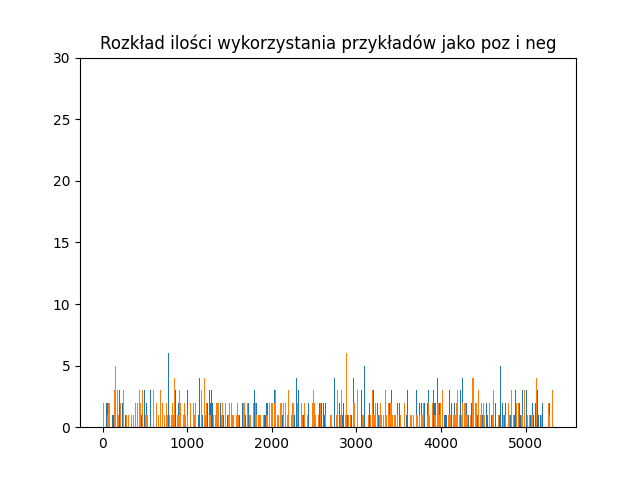
\includegraphics[width=0.8\linewidth]{figures/semantics/labse_output.png}
    \caption{Ilości reprezentacji przykładów jako pozytywne i negatywne dla modelu Labse w ramach zbioru \textit{Medical Speech, Transcription, and Intent}. Kolorem pomarańczowym oznaczono ilość zdań, dla których dany przykład jest przykładem negatywnym, niebieskim -- pozytywnym}
    \label{fig:latent:labseDistribution}
\end{figure}

\begin{figure}
    \centering
    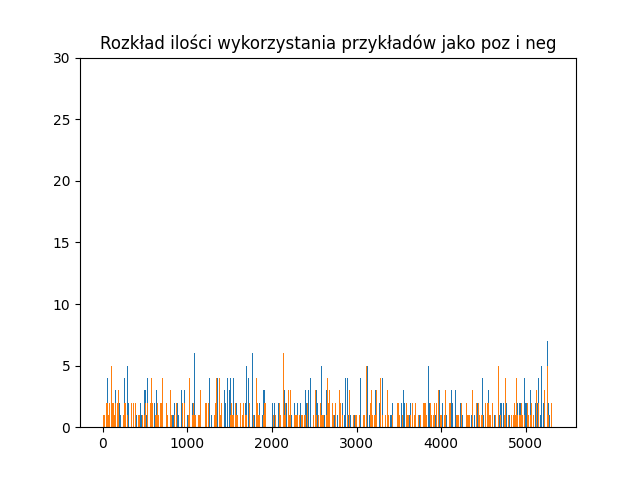
\includegraphics[width=0.8\linewidth]{figures/semantics/fleurs_labse_output.png}
    \caption{Ilości reprezentacji przykładów jako pozytywne i negatywne dla modelu Labse w ramach zbioru FLEURS. Kolorem pomarańczowym oznaczono ilość zdań, dla których dany przykład jest przykładem negatywnym, niebieskim -- pozytywnym}
    \label{fig:latent:labseDistributionFleurs}
\end{figure}

Rozkłady przykładów $x^n$ i $x^p$, dzięki zastosowaniu losowego wyboru były dosyć równomierne dla obu zbiorów danych, co przedstawiono na rysunkach \ref{fig:latent:labseDistribution} i \ref{fig:latent:labseDistributionFleurs}.

\subsubsection{Implementacja}
Eksperymenty zostały przeprowadzone z wykorzystaniem języka Python w wersji 3.12. Modele ASR i embeddingowe wraz z ich wagami zostały pobrane ze strony HuggingFace za pomocą bibliotek \textit{transformers} i \textit{sentence-transformers}. Do szybkiego obliczenia odległości między embeddingami wraz z wyłonieniem najbliższych i najdalszych embeddingów wykorzystaliśmy biblioteki \textit{Pytorch} i \textit{keOps}. Do obliczeń pomocniczych wykorzystaliśmy bibliotekę \textit{numpy}, natomiast do wizualicji -- \textit{matplotlib}. Eksperyment przeprowadzony został na serwerze obliczeniowym przy użyciu karty graficznej Nvidia RTX A5000.
\subsubsection{Analiza wyników}

\paragraph{Analiza enkodowania znaczenia semantycznego mowy}

Rozkłady wartości metryki $S(x_{emb,asr})$ (równanie \ref{eq:tripletDiff}) dla poszczególnych modeli ASR przedstawione są na wykresach zamieszczonych w sekcji Dodatki.

Tabela \ref{tab:latent:haniaCounts} przedstawia ilość przykładów w ramach zbioru danych \textit{Medical Speech, Transcription, and Intent}, dla których metryka $S(x_{emb,asr})$ przyjmowała wartości dodatnie, czyli tam, gdzie model ASR z powodzeniem uchwycił relacje semantyczne. Widać na niej wyraźną przewagę modelu SeamlessM4T, jak i dobre wyniki dla modeli Whisper i Hubert, które uchwyciły podobieństwo dla podobnie wysokiej liczby przykładów w ramach tego zbioru danych.

Tabela \ref{tab:latent:haniaDist} ilustruje z kolei parametry dopasowanego przez nas rozkładu Student-t dla zagregowanych różnic podobieństwa w ramach wszystkich modeli embeddingowych. Liczba stopni swobody $\nu$ odpowiedzialna jest za opisanie stabilności rozkładu w świetle obecności ogonów - im większa, tym bardziej stabilny jest rozkład. Wartości zbliżone do 2, jakie otrzymaliśmy dla modeli Data2Vec, Wav2Vec i Whisper wskazują na ich wysoką niestabilność w uchwyceniu relacji semantycznych. SeamlessM4T okazuje się najbardziej przewidywalnie zachowującym się modelem, dla którego $\nu = 6.4$, znacznie przewyższając drugi najwyżej plasujący się model HuBERT ($\nu = 3.6$). Znormalizowana lokalizacja ($\mu/\sigma$) pozwala nam na porównanie separacji pozytywnych i negatywnych przykładów między ewaluowanymi modelami ASR (MMD nie zachowuje skali pomiędzy modelami). Po raz kolejny, model SeamlessM4T wykazuje się najsilniejszą zdolnością rozróżniania przykładów pozytywnych i negatywnych ($\mu/\sigma = 0.91$). Modele HuBERT i Whisper osiągneły wyniki blisko dwukrotnie gorsze ($\mu/\sigma = 0.61$ i $\mu/\sigma = 0.54$), natomiast Data2Vec i Wav2Vec przejawiają podobnie niską zdolność dyskryminacji ($\mu/\sigma \approx 0.33$). Ostatnią z badanych metryk jest prawdopodobieństwo prawidłowego uchwycenia relacji między $x^a$, $x^n$ i $x^p$. Jest ona podobna do podejścia stricte ilościowego, lecz pozwala ona również analizować osiągi modelu w świetle dopasowanego przez nas rozkładu. Podobnie jak w porównaniu ilościowym, SeamlessM4T deklasuje resztę modeli, natomiast zarówno Whisper jak i HuBERT wykazują podobnie dobre wyniki. Warto zauważyć jednak, że HuBERT osiąga lepsze wyniki dla tej metryki ($P(neg > pos) = 71\%$) niż Whisper ($P(neg>pos) = 67.8\%$), wskazując na przewagę tego modelu, niewidoczną dla porównania ilościowego, która spowodowana jest prawdopodobnie większą stabilnością dopasowanego rozkładu.

\begin{table}[ht]
\centering
\caption{$S(x_{emb,asr}) > 0$ dla zbioru \textit{Medical Speech, Transcription, and Intent} (Ilość przykładów = 5327)}
\label{tab:latent:haniaCounts}
\begin{tabular}{lccc}
\toprule
\textbf{Model} & \textbf{Jina} & \textbf{LaBSE} & \textbf{SBERT} \\
\midrule
Wav2Vec  & 3352 & 3377 & 3472 \\
Data2Vec & 3290 & 3337 & 3375 \\
M4T  & \textbf{4375} & \textbf{4443} & \textbf{4413} \\
Whisper  & 3848 & 4006 & 3802 \\
HuBERT   & 3801 & 3971 & 3827 \\
\bottomrule
\end{tabular}
\end{table}

\begin{table}[t]
\centering
\begin{tabular}{lccc}
\hline
Model & Liczba stopni swobody ($\nu$) & Znormalizowana lokalizacja ($\mu/\sigma$) & $P(\text{neg} > \text{pos})$ \\
\hline
Data2Vec  & 2.1 & 0.32 & 61.1\% \\
Wav2Vec   & 2.3 & 0.35 & 62.1\% \\
M4T    & \textbf{6.4} & \textbf{0.98} & \textbf{81.8\%} \\
Whisper   & 1.9 & 0.54 & 67.8\% \\
HuBERT    & 3.6 & 0.61 & 71.0\% \\
\hline
\end{tabular}
\caption{Parametry rozkładów Student-$t$ dopasowanych do zagregowanych krzywych różnicy podobieństwa dla zbioru \textit{Medical Speech, Transcription, and Intent}}
\label{tab:latent:haniaDist}
\end{table}

Wyniki dla dwujęzycznej wersji zbioru Fleurs (język polski i angielski) zostały przedstawione dla modeli ASR wspierających oba z tych języków, reprezentujące trzy rodziny modeli - HuBERT (mHuBERT), Whisper i SeamlessM4T. Rozkłady dla tych modeli przedstawione zostały na rysunkach zamieszczonych w sekcji Dodatki. Tabele \ref{tab:latent:fleursCounts} i \ref{tab:latent:fleursDist} przedstawiają ilościowe porównanie wyników eksperymentu.

\begin{table}[ht]
\centering
\caption{$S(x_{emb,asr}) > 0$ dla zbioru \textit{Fleurs} (Ilość przykładów = 5443)}
\label{tab:latent:fleursCounts}
\begin{tabular}{lccc}
\toprule
\textbf{Model} & \textbf{Jina} & \textbf{LaBSE} & \textbf{SBERT} \\
\midrule
M4T  & \textbf{4256} & \textbf{4284} & \textbf{3911} \\
Whisper  & 3918 & 3895 & 3295 \\
HuBERT  & 3650 & 3721 & 3295 \\
mHuBERT   & 3296 & 3430 & 3288 \\
\bottomrule
\end{tabular}
\end{table}

\begin{table}[t]
\centering
\begin{tabular}{lccc}
\hline
Model & Liczba stopni swobody ($\nu$) & Znormalizowana lokalizacja ($\mu/\sigma$) & $P(\text{neg} > \text{pos})$ \\
\hline
M4T    & 6.8 & \textbf{0.72} & \textbf{75.3\%} \\
Whisper   & \textbf{10.4} & 0.49 & 68.3\% \\
HuBERT   & 8.3 & 0.40 & 64.9\% \\
mHuBERT    & 2.8 & 0.27 & 59.6\% \\
\hline
\end{tabular}
\caption{Parametry rozkładów Student-$t$ dopasowanych do zagregowanych krzywych różnicy podobieństwa dla zbioru \textit{Fleurs}}
\label{tab:latent:fleursDist}
\end{table}

Zarówno na podstawie Tabeli \ref{tab:latent:fleursCounts} jak i Tabeli \ref{tab:latent:fleursDist} zauważyć można dużą przewagę modelu M4T nad pozostałymi modelami. Zarówno umiejętność poprawnej separacji przykładów negatywnych i pozytywnych ($\mu/\sigma$ = 0.72), średnia ilość poprawnie przyporządkowanych przykładów ($E[n_\text{poz}] = 4150$), jak i prawdopodobieństwo poprawnego przyporządkowania przykładów ($P(\text{neg} > \text{poz}) = 75.3\%$) stawiają SeamlessM4T jako model najlepiej enkodujący semantykę wypowiedzi. Wyniki dla modelu Whisper również wskazują na enkodowanie przez niego znaczenia treści danych wejściowych, z gorszą zdolnością separacji przykładów ($\mu/\sigma$ = 0.49) i prawdopodobieństwem prawidłowego ich przyporządkowania ($P(\text{neg} > \text{poz}) = 68.3\%$), lecz z bardziej stabilnym rozkładem przypadków ($\nu = 10.4$) w porównaniu z SeamlessM4T ($\nu = 6.8$), co wskazuje na zadowalające zdolności modelu Whisper do reprezentacji semantyki danych wejściowych. Zdecydowanie najgorzej wypadł w tym porównaniu model mHuBERT, który z niskim prawdopodobieństwem poprawnie klasyfikował znaczenie danych wejściowych w świetale ich semantyki ($P(\text{neg} > \text{poz}) = 59.6\%$), osiągając wyniki niewiele większe niż wybór losowy i gorsze niż bazowy model HuBERT($P(\text{neg} > \text{poz}) = 64.5\%$). Możliwą przyczyną tak niskiego wyniku jest niska elastyczność modelu, stworzonego oryginalnie wyłącznie do transkrypcji mowy w języku angielskim, jak i mocy dekodera obecnego w pełnej propagacji w przód modelu. Kolejnym wyjaśnieniem jest zakłócenie oryginalnie silnej reprezentacji semantycznej w modelu angielskim (model HuBERT dla zbioru \textit{Medical Speech, Transcription, and Intent}, tabela \ref{tab:latent:haniaDist}) przez dotrenowanie na danych ze 146 kolejnych języków, przez które model o tak małej liczbie parametrów -- 94.4 miliona -- musiał enkodować tekst wejściowy w pewien bardziej skompresowany sposób, nie nadający się do interpretacji w świetle semantyki embeddingów. Hipotezę tę potwierdzają wyniki pracy \textit{Adapting multilingual speech representation model for a new, underresourced language through multilingual fine-tuning and continued pretraining}, w której autorzy zauważyli wyraźnie gorsze wyniki modelu dotrenowanego do transkrypcji języka Ainu na danych w języku angielskim (językowo bardzo różnym od Ainu) \cite{latentBreakMultilingual}. Wskazuje to na wysokie prawdopodobieństwo wystąpienia zjawiska zapominania (\textit{catastrophic forgetting}), analiza którego nie została umieszczona w oryginalnej pracy autorów mHuBERT-147 \cite{mhubert}.

Warto zwrócić uwagę na parametr $\nu$ opisujący stabilność rozkładu, który największa wartość przyjmuje dla modelu Whisper, w porównaniu do jego wartości dla zbioru \textit{Medical Speech, Transcription, and Intent} - dla zbioru \textit{Fleurs} modele o wiele lepiej radzą sobie z ekstremalnymi przypadkami odległości przykładów \textit{anchor}, \textit{pos} i \textit{neg}. Jest to najprawdopodobniej spowodowane kombinacją dwóch czynników -- sztucznej separacji przestrzeni embeddingowej między dwoma językami, która w mniejszym lub większym stopniu jest obecna w każdym z badanych modeli jak i szerszą domeną samego zbioru danych \textit{Fleurs}, który nie skupia się wyłącznie na tematycze medycznej.

%
% Cone
%
\paragraph{Analiza efektu stożka dla wybranych wielojęzycznych modeli ASR}

\begin{figure}
    \centering
    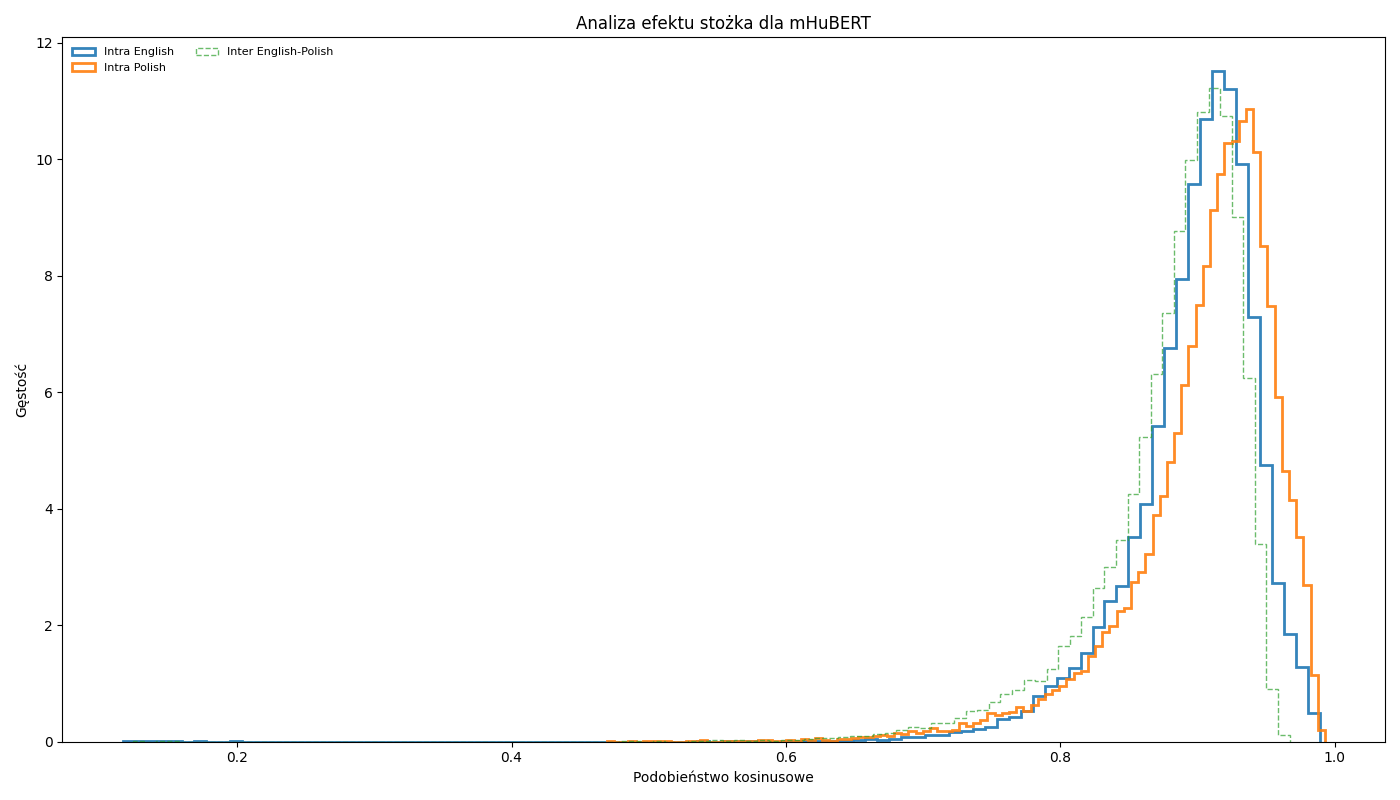
\includegraphics[width=0.8\linewidth]{figures/semantics/mhubert_cone.png}
    \caption{Gęstość podobieństwa kosinusowego z uwzględnieniem języków dla mHuBERT w ramach zbioru \textit{Fleurs}}
    \label{fig:latent:coneMHubert}
\end{figure}

\begin{figure}
    \centering
    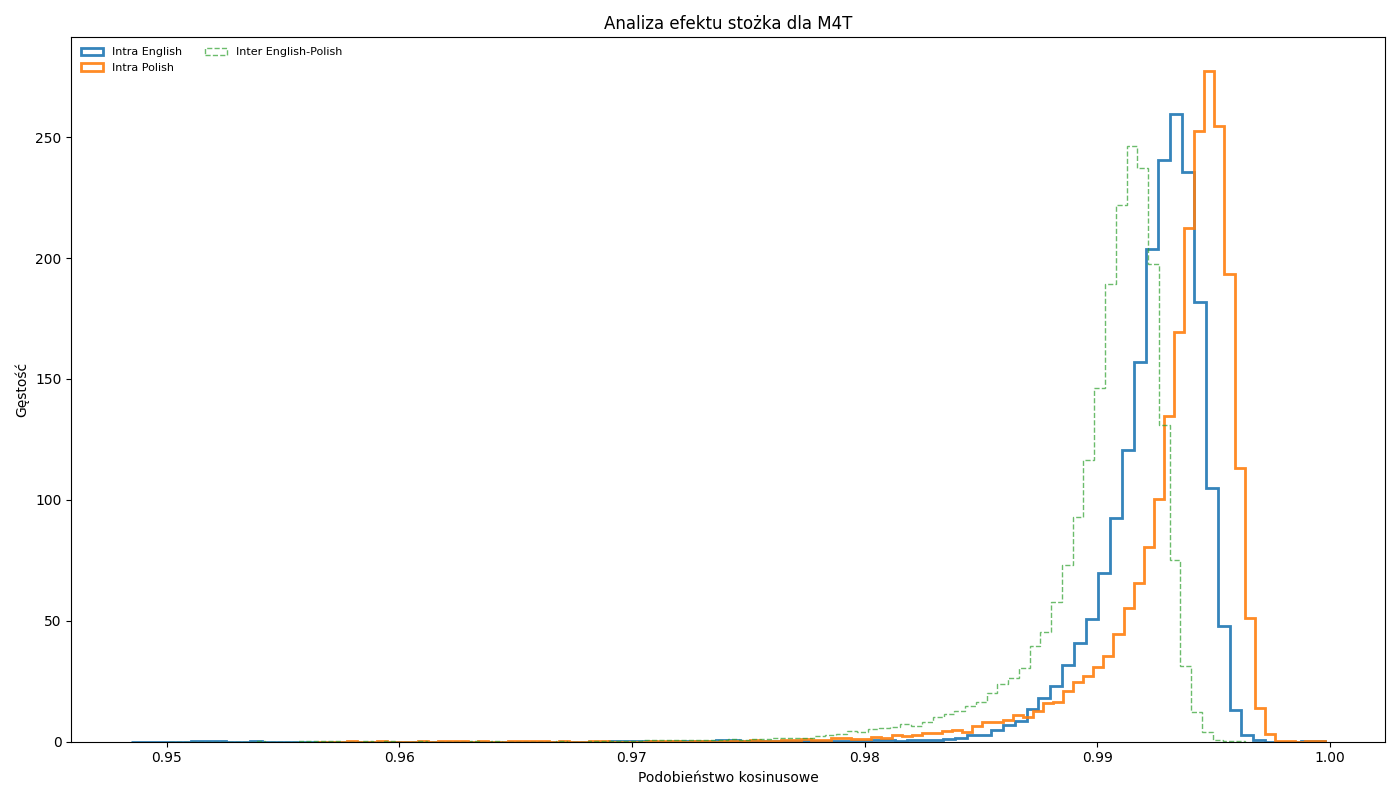
\includegraphics[width=0.8\linewidth]{figures/semantics/m4t_cone.png}
    \caption{Gęstość podobieństwa kosinusowego z uwzględnieniem języków dla M4T w ramach zbioru \textit{Fleurs}}
    \label{fig:latent:coneM4T}
\end{figure}

\begin{figure}
    \centering
    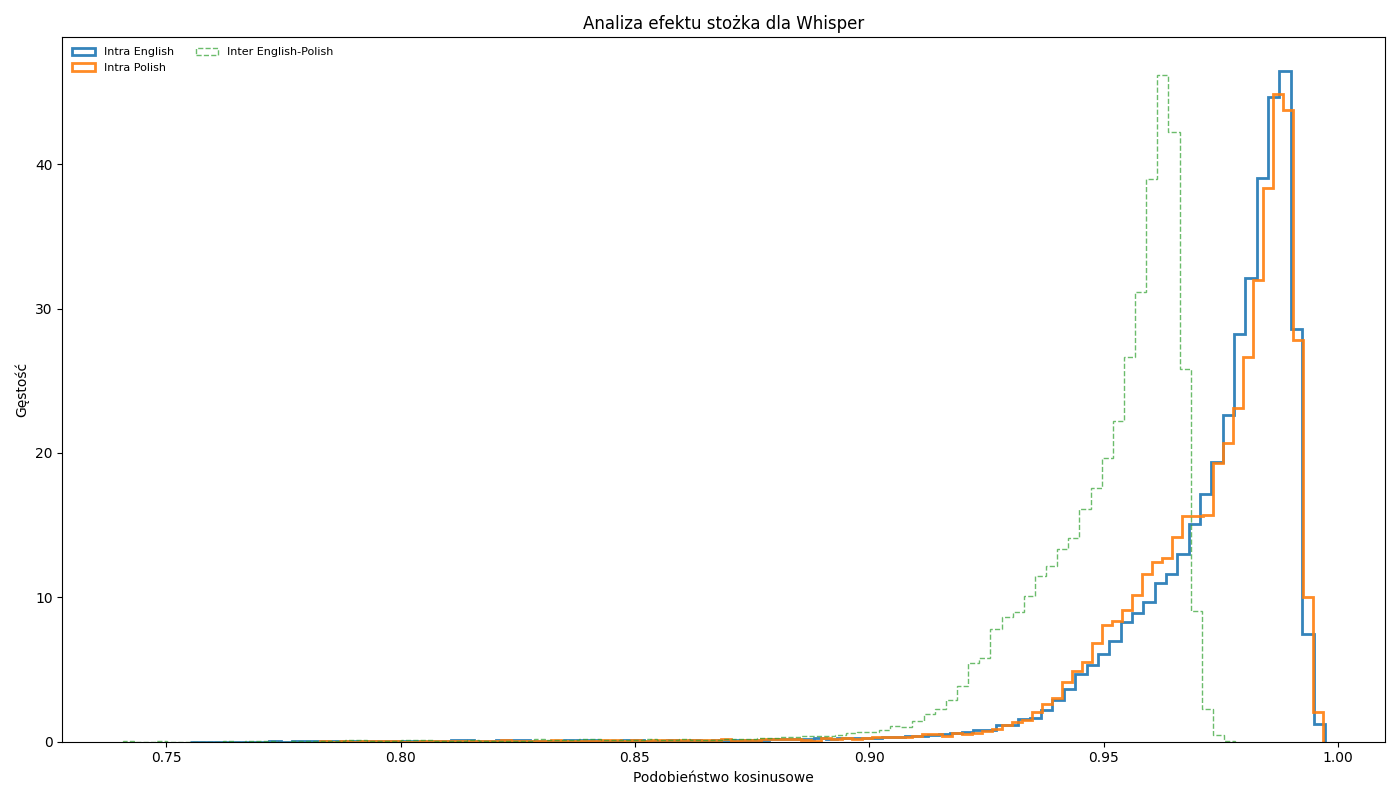
\includegraphics[width=0.8\linewidth]{figures/semantics/whisper_cone.png}
    \caption{Gęstość podobieństwa kosinusowego z uwzględnieniem języków dla Whisper w ramach zbioru \textit{Fleurs}}
    \label{fig:latent:coneWhisper}
\end{figure}

Wykresy gęstości podobieństwa kosinusowego dla zbioru \textit{Fleurs} w zależności od języków przedstawione zostały na rysunkach \ref{fig:latent:coneMHubert}, \ref{fig:latent:coneM4T} i \ref{fig:latent:coneWhisper}


Widoczny jest tutaj wyraźnie fenomen stożka, zgodny z zależnością zaobserwowaną w pracy \textit{How Contextual are Contextualized Word Representations? Comparing the Geometry of BERT, ELMo, and GPT-2 Embeddings}, w której autor zauważył wzrost anizotropi przestrzeni ukrytych modeli językowych wraz ze wzrostem ilości warstw \cite{cone} -- wraz ze wzrostem liczby parametrów i warstw, reprezentacje latentne zajmują coraz to mniejszy fragment przestrzeni (rozkład dla mHuBERT -- 94.4 miliona parametrów [rysunek \ref{fig:latent:coneMHubert}] a ten sam rozkład dla SeamlessM4T -- 2 miliardy parametrów [rysunek \ref{fig:latent:coneM4T}]). W celu stwierdzenia czy reprezentacje mowy wymawianej w różnych językach tworzą osobne klastry w przestrzeni embeddingowej należy spojrzeć na odległość między wykresami gęstości dla podobieństw kosinusowych wewnątrz języków i między językami. Modele mHuBERT i SeamlessM4T wydają się enkodować informacje agnostycznie od języka, z separacją między grupami językowymi będącą wyraźnie najmniejszą dla pierwszego modelu (częściowe pokrycie i niewielkie przesunięcie gęstości między grupami a wewnątrz grup na rysunkach \ref{fig:latent:coneMHubert} i \ref{fig:latent:coneM4T}). Model Whisper wykazuje dosyć dużą separację między grupami językowymi w ramach reprezentacji latentnych (rysunek \ref{fig:latent:coneWhisper}). Właściwość ta może prowadzić do mniej dokładnego wyszukiwania informacji między językami polskim i angielskim, a także do gorszego transferu wiedzy pozyskanej w ramach treningu na specjalistycznych zbiorach w języku angielskim do analogicznej wiedzy w języku polskim.

\begin{figure}
    \centering
    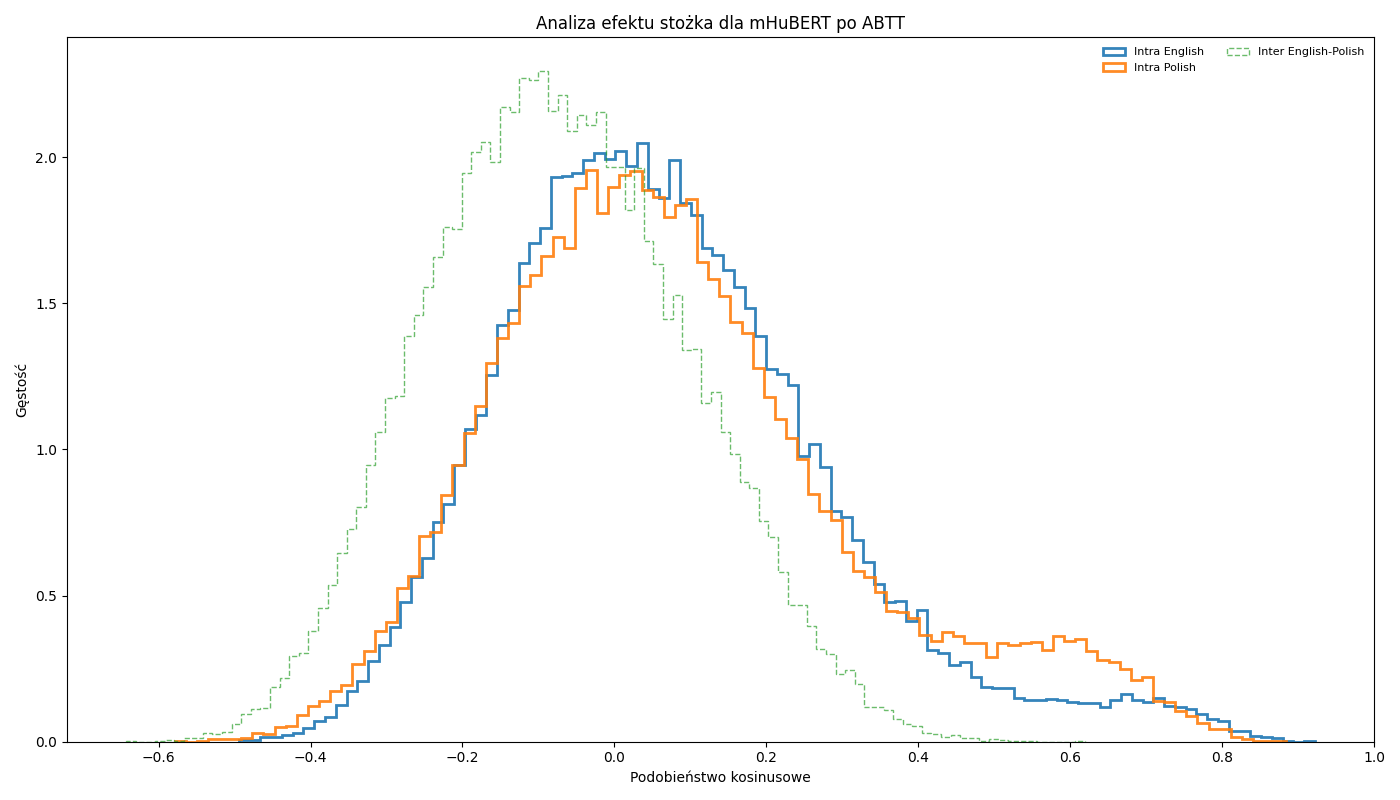
\includegraphics[width=0.8\linewidth]{figures/semantics/mhubert_cone_abtt.png}
    \caption{Gęstość podobieństwa kosinusowego z uwzględnieniem języków dla MHuBERT w ramach zbioru \textit{Fleurs} po transformacji ABTT}
    \label{fig:latent:coneMhubertAbtt}
\end{figure}

\begin{figure}
    \centering
    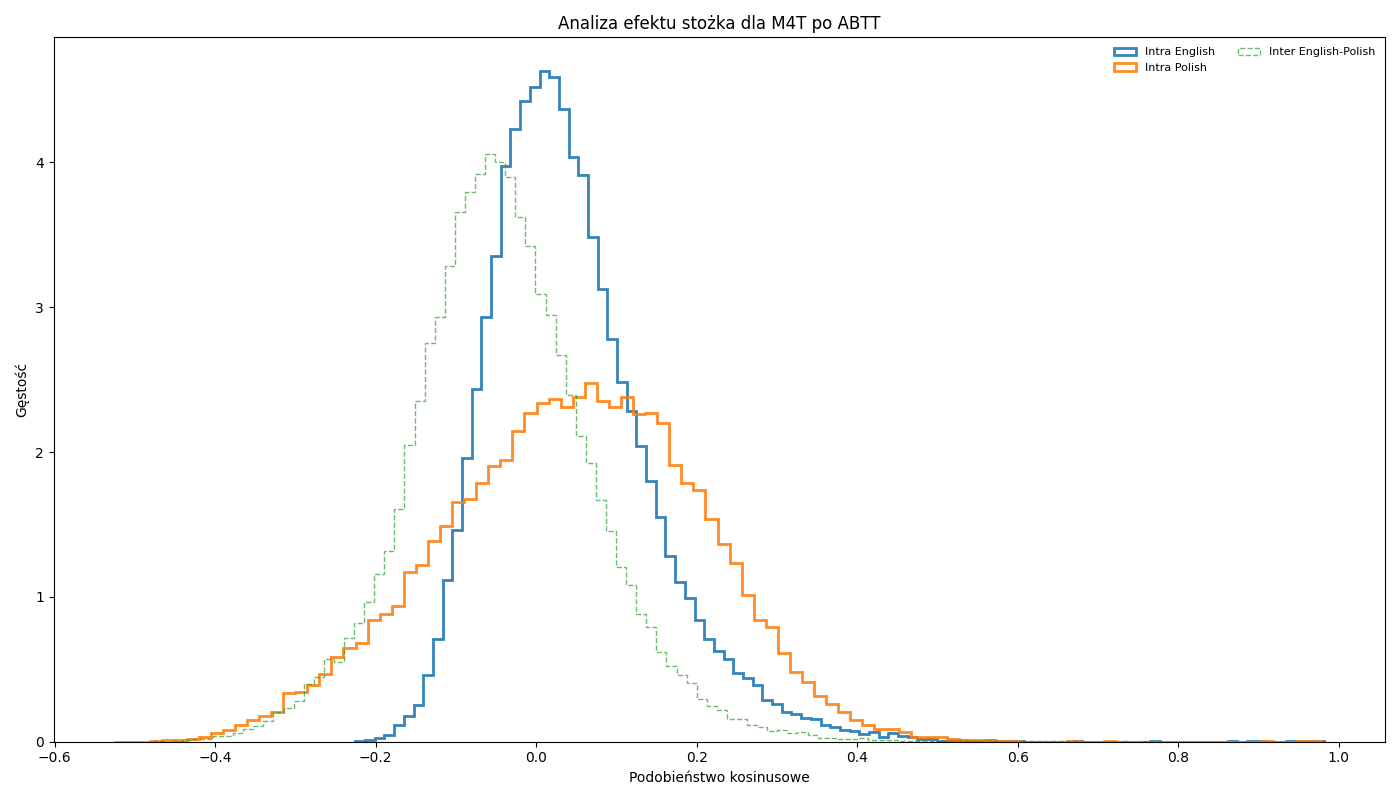
\includegraphics[width=0.8\linewidth]{figures/semantics/m4t_cone_abtt.png}
    \caption{Gęstość podobieństwa kosinusowego z uwzględnieniem języków dla M4T w ramach zbioru \textit{Fleurs} po transformacji ABTT}
    \label{fig:latent:coneM4TAbtt}
\end{figure}

\begin{figure}
    \centering
    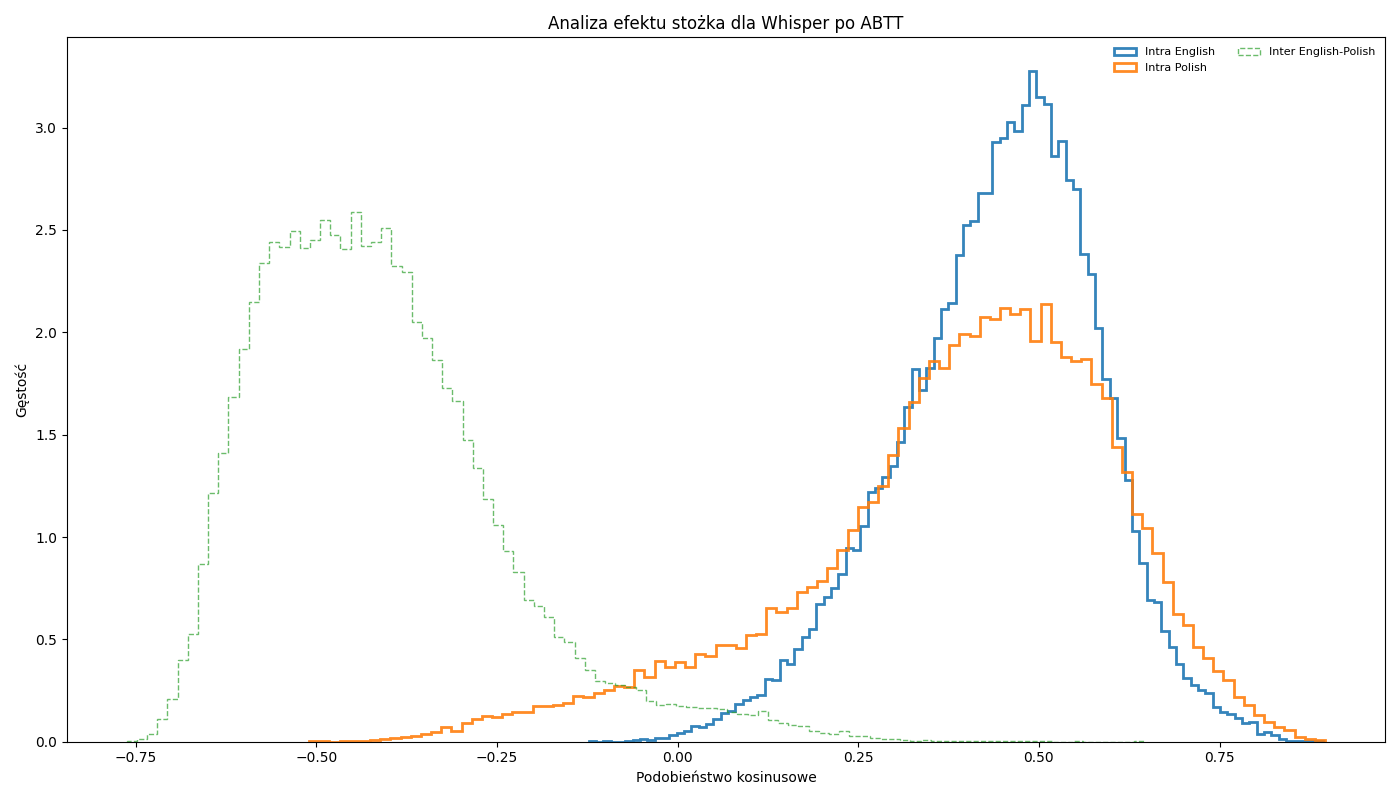
\includegraphics[width=0.8\linewidth]{figures/semantics/whisper_cone_abtt.png}
    \caption{Gęstość podobieństwa kosinusowego z uwzględnieniem języków dla Whisper w ramach zbioru \textit{Fleurs} po transformacji ABTT}
    \label{fig:latent:coneWhisperAbtt}
\end{figure}

Rysunki \ref{fig:latent:coneMhubertAbtt}, \ref{fig:latent:coneM4TAbtt} i \ref{fig:latent:coneWhisperAbtt} przedstawiają rozkłady gęstości podobieństwa kosinusowego między embeddingami po przekształceniu \textit{All But the Top}. Dla wszystkich modeli, badane reprezentacje latentne zajęły większą część dostępnej przestrzeni. Jest to spowodowane usunięciem pierwszej głównej składowej po analizie PCA, dzięki czemu pewne wspólne informacje przechowywane przez reprezentacje latentne zostały odrzucone, pozostawiając wyłącznie cechy własne charakteryzujące dane wejściowe. Model mHuBERT (rysunek \ref{fig:latent:coneMhubertAbtt}) zachował prawie identyczne rozkłady w ramach grup językowych, z gęstością podobieństwa lekko przesuniętą. Wskazuje to na większą separację grup językowych niż w ramach danych nieprzetworzonych (rysunek \ref{fig:latent:coneMHubert}). Może być to spowodowane tendencją modelu do enkodowania informacji dotyczących języka, w niewielkim stopniu, na przykład informacji prozodycznych. Seamless M4T wykazuje się podobną charakterystyką co do przesunięcia podobieństwa między grupami, które było obecne również dla danych nieprzetworzonych (rysunki \ref{fig:latent:coneM4TAbtt} i \ref{fig:latent:coneM4T}). Warto zwrócić uwagę na różnicę rozkładów wewnątrz grup językowych -- embeddingi dla języka polskiego zajmują o wiele większą część przestrzeni niż embeddingi dla języka angielskiego. Naszą hipotezą jest obecność pewnego meta-języka opisującego dane dla modelu M4T, który podobny jest najbardziej do języka angielskiego. O ile autorzy modelu nie podali dokładnego balansu danych między różnymi językami w ramach danych treningowych modelu \cite{m4t}, można przypuszczać dominację danych w języku angielskim, stąd też bardziej dokładne reprezentacje danych w języku angielskim. Charakterystyka modelu Whisper (rysunek \ref{fig:latent:coneWhisperAbtt}) zaobserwowana dla danych nieprzetworzonych (rysunek \ref{fig:latent:coneWhisper}) została potwierdzona przez rozkłady dla embeddingów po przetworzeniu \textit{All But the Top}. Widoczna jest o wiele bardziej wyraźna separacja na pewne klastry reprezentujące języki polski i angielski. Jest to najprawdopodobniej spowodowane charakterystyką treningu, w ramach której funkcja straty nie wymusza w jakikolwiek sposób współdzielenia przestrzeni latentnej przez dane z różnych języków, dane treningowe dla transkrypcji precyzują język wypowiedzi \cite{whisper}.

\begin{figure}
    \centering
    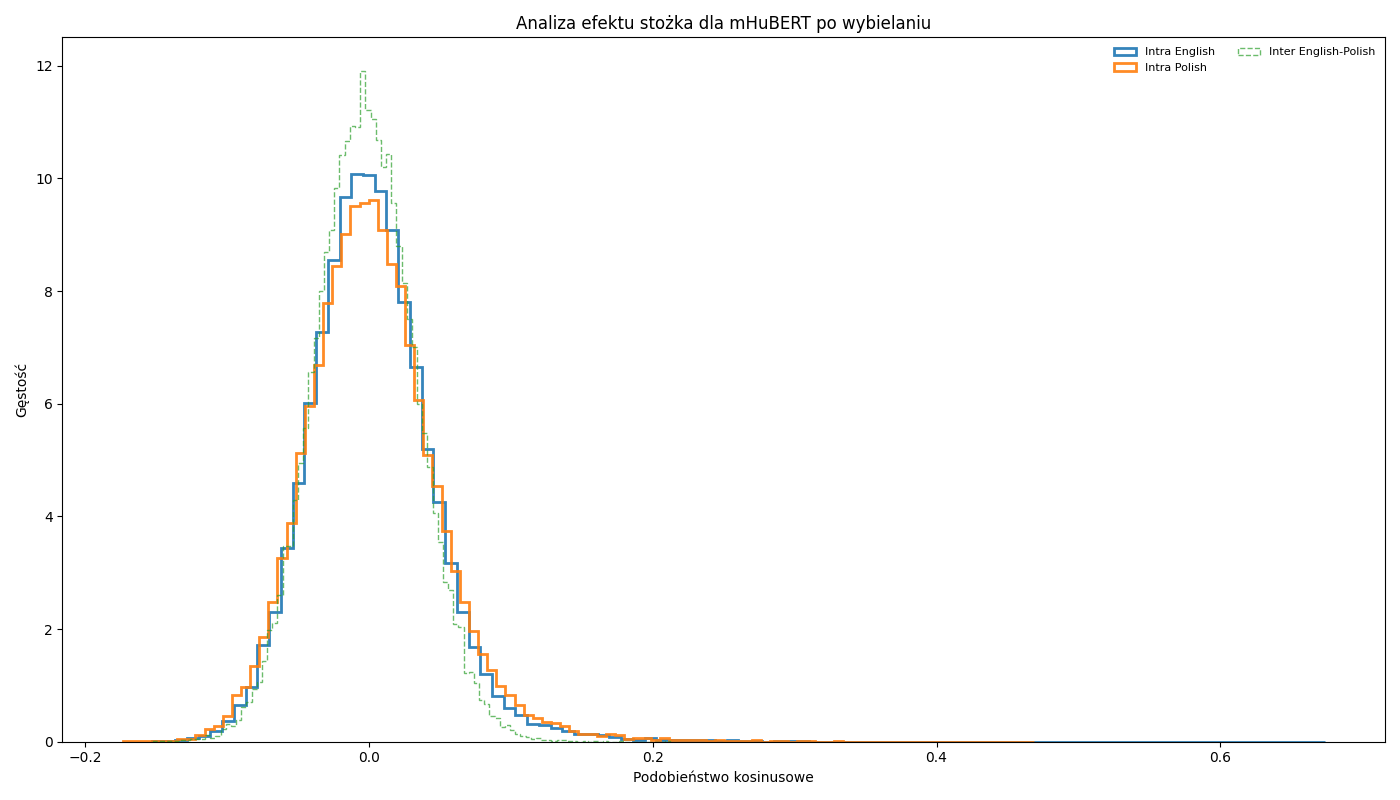
\includegraphics[width=0.8\linewidth]{figures/semantics/mhubert_cone_whitened.png}
    \caption{Gęstość podobieństwa kosinusowego z uwzględnieniem języków dla MHuBERT w ramach zbioru \textit{Fleurs} po wybielaniu}
    \label{fig:latent:coneMhubertWhitened}
\end{figure}

\begin{figure}
    \centering
    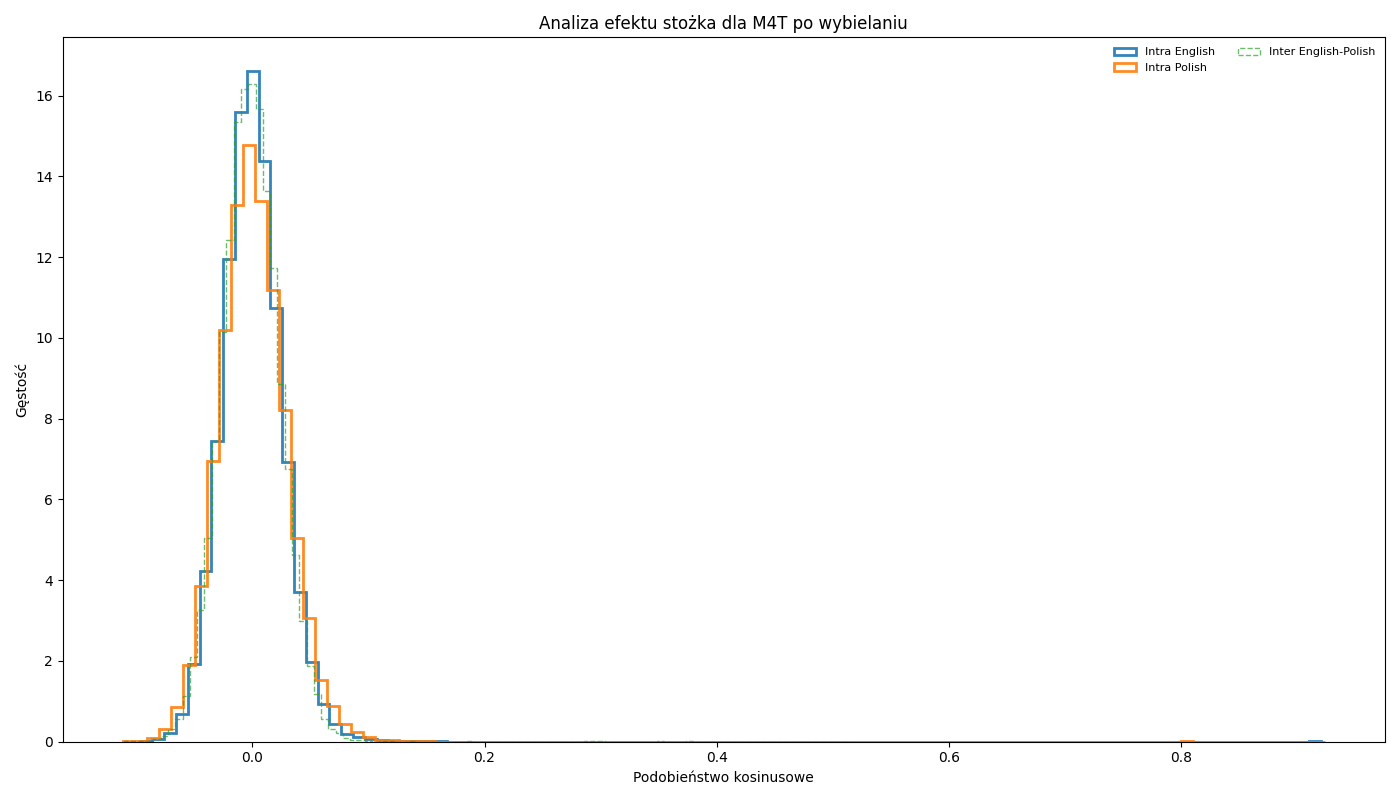
\includegraphics[width=0.8\linewidth]{figures/semantics/m4t_cone_wnitened.png}
    \caption{Gęstość podobieństwa kosinusowego z uwzględnieniem języków dla M4T w ramach zbioru \textit{Fleurs} po wybielaniu}
    \label{fig:latent:coneM4TWhitened}
\end{figure}

\begin{figure}
    \centering
    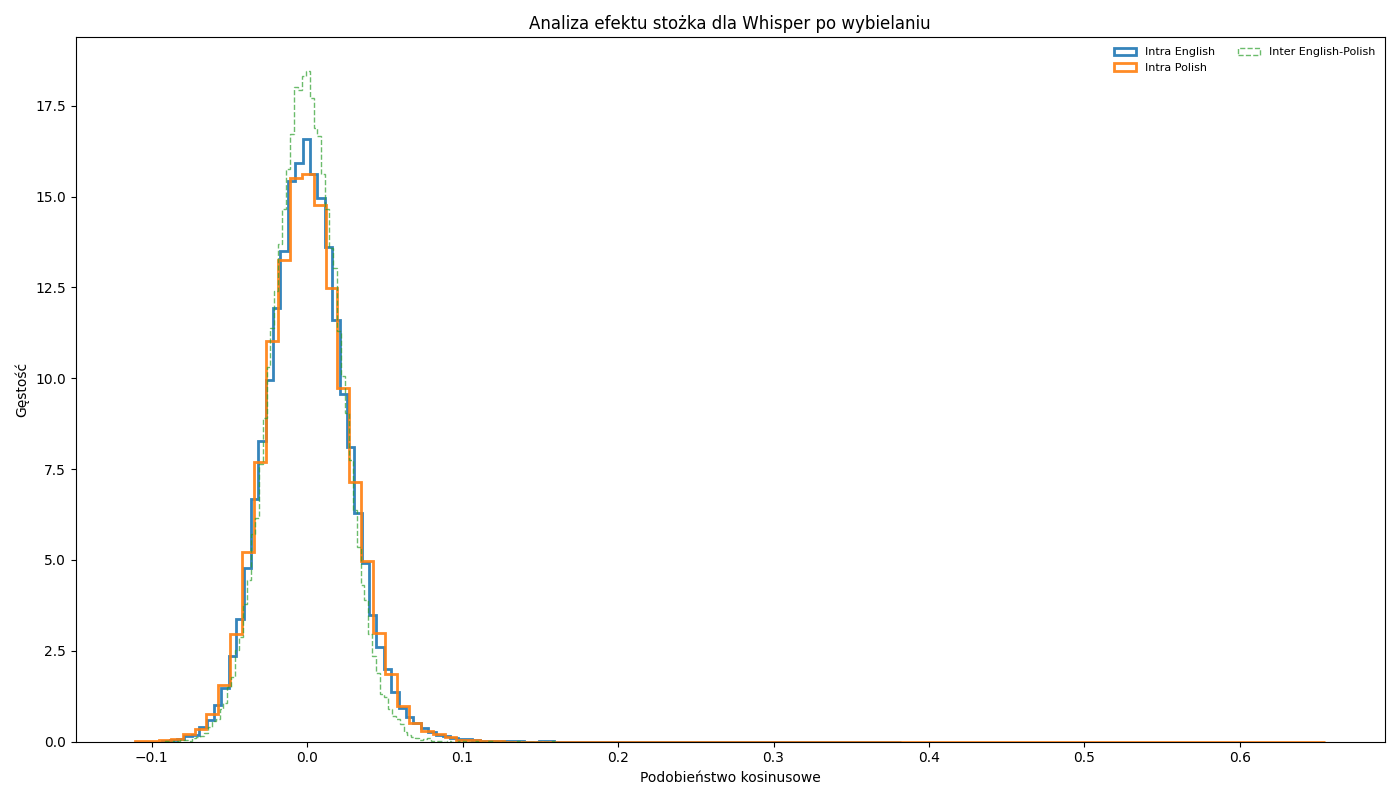
\includegraphics[width=0.8\linewidth]{figures/semantics/whisper_cone_wnitened.png}
    \caption{Gęstość podobieństwa kosinusowego z uwzględnieniem języków dla Whisper w ramach zbioru \textit{Fleurs} po wybielaniu}
    \label{fig:latent:coneWhisperWhitened}
\end{figure}

Rysunki \ref{fig:latent:coneMhubertWhitened}, \ref{fig:latent:coneM4TWhitened} i \ref{fig:latent:coneWhisperWhitened} przedstawiają rozkłady podobieństwa kosinusowego po przeprowadzeniu wybielania (\textit{whitening}). Dzięki dekorelacji danych w ramach tego procesu, widoczna jest tutaj bliska idealnej umiejętność łączenia języków w jedną grupę, co prowadzi do dobrego transferu wiedzy między językami. Jednakże, w porównaniu z rozkładami dla przetwarzania ABTT, widoczne jest pewne zawężenie przestrzeni embeddingowej -- efekt stożka jest bardziej widoczny. Mimo tego, w świetle reprezentacji bazowych, embeddingi zajmują o wiele większy odsetek dostępnej przestrzeni.

Podsumowując, zabieg ABTT zdecydowanie poprawił ogólny rozkład embeddingów w przestrzeni, nie do końca redukując (a dla modelu Whisper pogłębiając) separację między reprezentacjami różnych języków. Wybielanie pozwoliło również na redukcję efektu stożka, tym samym dekorelując embeddingi w świetle języka, potencjalnie poprawiając transfer wiedzy w ramach treningu na danych w języku angielskim. Analiza ta wykazała poprawność wykorzystania postprocsessingu w świetle niwelowania anizotropi reprezentacji ukrytych dla modeli ASR.

\paragraph{Analiza wpływu przetwarzania embeddingów na zachowanie semantyki}
Oprócz modeli poddanych analizie w ramach badania efektu stożka, tj. Whisper, mHuBERT i SeamlessM4T, w tym eksperymencie uwzględniliśmy róznież bazowy model HuBERT, który wykazywał dobre wyniki w ramach zbiorów \textit{Medical Speech, Transcription, and Intent} i \textit{Fleurs}.

Tabele \ref{tab:latent:cosCompNu}, \ref{tab:latent:cosineComparisonSeparability} i \ref{tab:latent:cosComparisonProbability} ilustrują porównanie parametrów dopasowanych rozkładów Student-t między analizą za pomocą metryki MMD i podobieństwa kosinusowego, natomiast rysunki przedstawiające te rozkłady umieszczone zostały w sekcji Dodatki.
\begin{table}[h]
\centering
\begin{tabular}{lccc}
\toprule
Model & MMD ($\nu$) & Podobieństwo kosinusowe ($\nu$) & Zmiana (\%) \\
\midrule
M4T     & 6.8  & 4.7  & -30.9 \\
Whisper & \textbf{10.4} & 7.6  & -26.9 \\
HuBERT  & 8.3  & \textbf{24.8} & \textbf{+198.8} \\
mHuBERT & 2.8  & 4.2  & +50.0 \\
\bottomrule
\end{tabular}
\caption{Porównanie parametru $\nu$ dla rozkładów MMD i podobieństwa kosinusowego.}
\label{tab:latent:cosCompNu}
\end{table}

\begin{table}[h]
\centering
\begin{tabular}{lccc}
\toprule
Model & MMD ($\mu/\sigma$) & Podobieństwo kosinusowe ($\mu/\sigma$) & Zmiana (\%) \\
\midrule
M4T     & \textbf{0.72} & \textbf{1.11} & \textbf{+54.2} \\
Whisper & 0.49 & 0.52 & +6.1 \\
HuBERT  & 0.40 & 0.31 & -22.5 \\
mHuBERT & 0.27 & 0.32 & +18.5 \\
\bottomrule
\end{tabular}
\caption{Porównanie parametru $\mu/\sigma$ dla rozkładów MMD i podobieństwa kosinusowego.}
\label{tab:latent:cosineComparisonSeparability}
\end{table}

\begin{table}[h]
\centering
\begin{tabular}{lccc}
\toprule
Model & MMD ($P$) & Podobieństwo kosinusowe ($P$) & Zmiana (\%) \\
\midrule
M4T     & \textbf{75.3} & \textbf{83.9} & \textbf{+11.4} \\
Whisper & 68.3 & 69.2 & +1.3 \\
HuBERT  & 64.9 & 62.1 & -4.3 \\
mHuBERT & 59.6 & 61.9 & +3.9 \\
\bottomrule
\end{tabular}
\caption{Porównanie prawdopodobieństw poprawnego uchwycenia relacji między przykładami bazowym, pozytywnym i negatywnym (MMD vs podobieństwo kosinusowe).}
\label{tab:latent:cosComparisonProbability}
\end{table}

W tabeli \ref{tab:latent:cosCompNu} widoczna jest stabilizacja rozkładu dla modeli z rodziny BERT (zmiana o $198.8\%$ i $50.0\%$ dla HuBERT i mHuBERT), z destabilizacją dla dwóch pozostałych modeli. Tabele \ref{tab:latent:cosineComparisonSeparability} i \ref{tab:latent:cosComparisonProbability} wykazują widoczny trend poprawy zarówno zdolności separacji, jak i ogólnej zdolności dyskryminacji pozytywnych i negatywnych przykładów dla SeamlessM4T i Whisper, z większym wzrostem metryk dla pierwszego z nich (wzrost o $54.2\%$ w znormalizowanej lokalizacji, $11.4\%$ w prawdopodobieństwie poprawnego uchwycenia relacji). Jest to prawdopodobnie spowodowane uniwersalnością enkodera SeamlessM4T, gdzie cały model wspiera modalności tekstu i mowy, przez co relacje czasowe muszą być zunifikowane w ramach tokenów tekstu i mowy. Whisper natomiast wykorzystuje najprawdopodobniej pewne zależności czasowe samej mowy, przez co usunięcie domeny czasu wiąże się z większą stratą informacji niż dla SeamlessM4T. Podobna właściwość modeli z rodziny BERT może stanowić również wyjaśnienie ich zachowania po usunięciu informacji z domeny czasu - zarówno mHuBERT, jak i HuBERT wykazują prawie identyczne właściwości względem separacji i zdolności poprawnej dyskryminacji rozkładu. Możliwe jest, że uśrednianie tokenów prowadzi do degradacji przestrzeni do prawie identycznej reprezentacji dla obu modeli.



Tabele \ref{tab:latent:compNu}, \ref{tab:latent:compLoc} i \ref{tab:latent:compProb} przedstawiają porównanie parametrów rozkładów dla embeddingów poddanych przetwarzaniu ABTT i wybielaniu. Wykresy przedstawiające te rozkłady zamieszczone zostały w sekcji Dodatki. Tabela \ref{tab:latent:processingCounts} przedstawia analizę ilościową poprawnie sklasyfikowanych przypadków. Ilości zostały uśrednione w ramach trzech różnych modeli embeddingowych.

\begin{table}[h]
\centering
\begin{tabular}{lccc}
\toprule
Model &
Podobieństwo kosinusowe &
ABTT &
Wybielanie \\
\midrule
M4T     & 4.7  & $1.96\times10^{10}$ & 0.8 \\
Whisper & 7.6  & $1.27\times10^{11}$ & 0.9 \\
HuBERT  & \textbf{24.8} & \textbf{$5.62\times10^{11}$} & 0.8 \\
mHuBERT & 4.2  & 5.2                 & \textbf{1.0} \\
\bottomrule
\end{tabular}
\caption{Porównanie parametru $\nu$ dla metod ABTT i wybielania względem bazowego podobieństwa kosinusowego.}
\label{tab:latent:compNu}
\end{table}

\begin{table}[h]
\centering
\begin{tabular}{lccccc}
\toprule
Model &
\multicolumn{1}{c}{Podobieństwo kosinusowe} &
\multicolumn{1}{c}{ABTT} &
\multicolumn{1}{c}{Zmiana (\%)} &
\multicolumn{1}{c}{Wybielanie} &
\multicolumn{1}{c}{Zmiana (\%)} \\
\midrule
M4T     & \textbf{1.11} & \textbf{1.41} & \textbf{+27.0} & 0.85 & -23.4 \\
Whisper & 0.52 & 0.44 & -15.4 & \textbf{0.95} & \textbf{+82.7} \\
HuBERT  & 0.31 & 0.34 & +9.7  & 0.52 & +67.7 \\
mHuBERT & 0.32 & 0.36 & +12.5 & 0.47 & +46.9 \\
\bottomrule
\end{tabular}
\caption{Porównanie parametru $\mu/\sigma$ dla metod ABTT i wybielania względem bazowego podobieństwa kosinusowego.}
\label{tab:latent:compLoc}
\end{table}

\begin{table}[h]
\centering
\begin{tabular}{lccccc}
\toprule
Model &
\multicolumn{1}{c}{Podobieństwo kosinusowe} &
\multicolumn{1}{c}{ABTT} &
\multicolumn{1}{c}{Zmiana (\%)} &
\multicolumn{1}{c}{Wybielanie} &
\multicolumn{1}{c}{Zmiana (\%)} \\
\midrule
M4T     & \textbf{83.9} & \textbf{92.1} & \textbf{+9.8} & 71.4 & -14.9 \\
Whisper & 69.2 & 67.1 & -3.0 & \textbf{73.1} & \textbf{+5.6} \\
HuBERT  & 62.1 & 63.3 & +1.9 & 64.5 & +3.9 \\
mHuBERT & 61.9 & 63.4 & +2.4 & 64.0 & +3.4 \\
\bottomrule
\end{tabular}
\caption{Porównanie prawdopodobieństwa poprawnego uchwycenia relacji między przykładami bazowym, pozytywnym i negatywnym dla metod ABTT i wybielania względem bazowego podobieństwa kosinusowego.}
\label{tab:latent:compProb}
\end{table}

\begin{table}[h]
\centering
\begin{tabular}{lccccc}
\toprule
Model &
Podobieństwo kosinusowe &
ABTT  &
Zmiana (\%) &
Wybielanie &
Zmiana (\%) \\
\midrule
M4T
& \textbf{4609} & \textbf{5131} & \textbf{+11.3} & \textbf{4915} & +6.6 \\
Whisper
& 3757 & 3816 & +1.6  & 4539 & \textbf{+20.8} \\
HuBERT
& 3474 & 3433 & -1.2  & 3951 & +13.7 \\
mHuBERT
& 3362 & 3402 & +1.2  & 3798 & +12.9 \\
\bottomrule
\end{tabular}
\caption{Średnia liczba poprawnych przypadków dla różnych embeddingów (Jina, LaBSE, SBERT) oraz względna poprawa metod ABTT i wybielania względem przypadku bazowego.}
\label{tab:latent:processingCounts}
\end{table}

Analizując Tabelę \ref{tab:latent:compNu}, zauważyć można popwawę stabilności rozkładu dla embeddingów poddanych przetwarzaniu ABTT dla wszystkich modeli. Jedynie mHuBERT nie osiągnął rozkładu praktycznie normalnego, lecz nadal cechuje się poprawą stabilności. Wybielanie doprowadziło z kolei do pewnej degradacji stabilności, uniwersalnie destabilizując wszytkie ewaluowane modele. Tak drastyczna różnica wynika zapewne z natury tych dwóch metod przetwarzania. O ile ABTT dokonuje wyłącznie projekcji do przestrzeni ortogonalnej do przestrzeni oryginalnej, o tyle wybielania prowadzi do rotacji i skalowania przestrzeni, mając o wiele większy wpływ na geometrię porównywanej przestrzeni, powodując odsunięcie się od rozkładu normalnego. Tabele \ref{tab:latent:compLoc} i \ref{tab:latent:compProb} pokazują zdolność separacji i prawdopodobieństwo poprawnego uchwycenia relacji przez modele. W modelach z rodziny HuBERT widoczna jest drastyczna poprawa zdolności separacji dla embeddingów poddanych wybielaniu ($67.7\%$ dla HuBERT, $46.9\%$ dla mHuBERT), jak i mniejsza, lecz zauważalna poprawa prawdopodobieństwa poprawnego uchwycenia badanej relacji ($3.9\%$ i $3.4\%$). Bardziej agresywna zmiana przestrzeni reprezentacji ukrytych poprawiła działanie tych modeli bardziej niż przekształcenie \textit{All But the Top}, które tylko nieznacznie poprawiło prawdopodobieństwo poprawnego przyporządkowania podobieństw przykładów. Mimo tego, modele te nie osiągnęły wyników większych niż wyniki bazowe dla modeli Whisper i SeamlessM4T. Dla tych dwóch modeli widoczna jest zgoła inna zależność i bardziej drastyczny wpływ doboru metody postprocessingu. SeamlessM4T poprawił swoje metryki o $27.0\%$ i $9.8\%$ dla ABTT, notując spadek dla bardziej agresywnej metody wybielania. Potencjalnym powodem są wysoka zdolność klasyfikacji semantycznej dla bazowego przypadku i zbyt duża modyfikacja geometrii przestrzeni po wykorzystaniu rotacji i skalowania, gdzie w przypadku ABTT informacje semantyczne nie są niszczone i poprawiana jest jedynie izotropia przestrzeni. Dla modelu Whisper ma miejsce zjawisko odwrotne -- to właśnie wybielanie poprawia wyniki modelu, a ABTT je redukuje. Negatywny wpływ metody \textit{All But the Top} powiązany może być z zachowaniem modelu w świetle efektu stożka przedstawionym na rysunku \ref{fig:latent:coneWhisperAbtt}, na którym wyraźnie widoczna jest separacja grup językowych, większa niż w przypadku nieprzetworzonych danych (rysunek \ref{fig:latent:coneWhisper}). Po wybielaniu modelu (rysunek \ref{fig:latent:coneWhisperWhitened}), w przestrzeni nie zauważono widocznych klastrów, co jest najbardziej prawdopodobnym powodem wzrostu badanych metryk. Jednakże, należy zauważyć wyraźną przewagę SeamlessM4T nad pozostałymi modelami, co potwierdza analiza ilościowa w tabeli \ref{tab:latent:processingCounts}. Nawet w ramach wybielania, które skutkuje spadkiem prawdopodobieństwa poprawnego uchwycenia relacji semantycznej o $14.9\%$, model ten poprawnie przyporządkował dane pod względem semantycznym większą ilość razy niż wszystkie inne badane modele.


\subsection{Podsumowanie i wnioski}
Wszystkie przeprowadzone przez nas eksperymenty wyraźnie wskazują na przewagę dwóch modeli ASR pod względem kodowania znaczenia semantycznego mowy -- SeamlessM4T i Whisper, dla których wyniki eksperymentów wskazują na kodowanie silnie nacechowanych semantycznie reprezentacji ukrytych. Pomimo potencjalnie bardziej stabilnego zachowania modeli z rodziny HuBERT, analiza ilościowa, jak i całościowa analiza parametrów dopasowanych rozkładów pokazały, że modele te nie są w stanie dorównać większym modelom w ramach wykorzystania ich jako enkoderów semantycznych cech mowy. Ponadto, wyniki wykazują pewną degradację semantyczności reprezentacji, nawet w ramach porównania na zbiorze wielojęzycznym, dla modelu mHuBERT w porównaniu z bazowym modelem HuBERT. Badając metody przetwarzania embeddingów, \textit{All But the Top} i wybielanie oparte na PCA, zauważyliśmy potencjalną poprawę reprezentacji, w szczególności dla modelów o wysokiej anizotropii przestrzeni, tj. SeamlessM4T i Whisper. Zmiany te jednak nadal nie podnoszą wyników mHuBERT i HuBERT na tyle, aby przewyższyć bazowe osiągi dwóch pozostałych modeli -- oznacza to, że dobór modelu ASR ma większe znaczenie niż dobór odpowiedniej metody przetwarzania embeddingów. Pokazaliśmy również poprawę reprezentacji względem grupowania reprezentacji danych wejściowych w języku polskim i angielskim, co umożliwi potencjalnie lepszy transfer wiedzy w ramach treningu na danych w obu tych językach.

Mając na uwadzę powyższe odkrycia, naturalnym wyborem do dalszej pracy nad modelami z rodziny speech-to-retrieval wydaje się być SeamlessM4T. Nie tylko uzyskiwał on najwyższe wyniki we wszystkich eksperymentach, lecz dzięki jego wsparciu dla modalności tekstowej, posiada on również swój dedykowany enkoder dla tekstu, który może być potencjalnie wykorzystany przy dalszym rozwoju naszych architektur. Kolejnym modelem wartym użycia jest Whisper, który w większości eksperymentów plasował się na drugiej pozycji. Dzięki wybielaniu, oryginalna reprezentacja wykazująca separację grup językowych ulega znormalizowaniu, umożliwiając naukę w na danych wielojęzycznych, jak i poprawia jakość semantycznego enkodowania reprezentacji danych wejściowych. Ponadto, model Whisper został sprawdzony w oryginalnej pracy ADMEDVoice \cite{ADMEDVoice} i może stanowić dobry punkt odniesienia dla naszych architektur.
